
\documentclass[aspectratio=169]{beamer}
\usepackage[utf8]{inputenc}
\usepackage[T1]{fontenc}
%%%%%%%
% \usepackage{layout}
% \usepackage{lipsum}
%%%%%%%
\usetheme[% Complete settings. Default value in []
% titleimagecolor=red,       % [gray], darkgray, red, blue, green
% titleimagemargin=2mm,      % Distance [2mm]    Frame around title page image
% navigationsymbols=false,   % true   / [false]  Navigation symbols in the foot
% mathseriffont=false,       % true   / [false]  Serif / non-serif math fonts
% foot=true,                 % [true] / false    Footline or not
% nofootslidenum=false       % true   / [false]  Keep slide num even when foot=false
% footlogo=true,             % [true] / false    Put LU logo to the left of footer
% english=true,              % [true] / false    English / Swedish logo
% LTHlogo=false,             % true   / [false]  Use LTH logo instead of LU on title and end pages.
% blackenumeratenumber=true, % [true] / false    Black enumerate numbers, o.w. Lund bronze
% blackitemmark=false,       % true   / [false]  Black item marks, o.w. Lund bronze
% defaultfont=false,         % true   / [false]  Falls back to default beamer fonts
% sectionframe=true,
]{ulund}
%%%%%%%%%%%%%%%%%%%%% Layout commands 
%%%% Foot
% \ulundfootleft{\insertshortauthor}
% \ulundfootmid{\insertshorttitle}
% \ulundfootright{\insertframenumber}% {\insertframenumber:\inserttotalframenumber}
%%%% Titleimage
\titleimage{Pictures/ULUNDcolor} % Replaces the LU image. Voids option titleimagecolor
%%%%%%%%%%%%%%%%%%%%%%%%%%%%%%%%%%%
\title[Scala First Lessons]{Scala First: \vspace{0.25em}\newline \fontsize{16}{25}\selectfont Lessons from 3 student generations }
\author[cs.lth.se/bjorn-regnell]{%
  Bjorn Regnell\newline
  Dept.\@ of Computer Science, Lund University}
%%%%%%%%%%%%%%%%%%%%%
%\usepackage{verbatim}
%%%%%%%%%%%%% Verbatim code box
\usepackage[skins,listings]{tcolorbox}
\tcbuselibrary{listingsutf8}

\usepackage{pgf-pie}

\newcommand{\Title}{\begin{frame}[plain]\titlepage\end{frame}}

\newcommand{\End}{\begin{frame}[plain]\endpage\end{frame}}


\newcommand{\Section}[1]{\titleimagecolor{red}\section{#1}}

\newenvironment{Slide}[1]%
  {\begin{frame}[environment=Slide]{#1}}
  {\end{frame}}%

\begin{document}

\Title

%%%%%%%%%%%%%%%

\begin{Slide}{Who is Bjorn Regnell?}
\begin{itemize}
\item Professor in Software Engineering
\item Dept. of Computer Science, Engineering Faculty LTH, Lund University, Sweden
\item Research focus: Software Requirements Engineering
\item Scala programmer since 2011 
\item Teaching Scala first in primary school since 2011
\item Teaching Scala first at university level since 2016
\item \textbf{\texttt{http://cs.lth.se/bjorn-regnell}}  
\end{itemize}  
\end{Slide}

\begin{Slide}{Scala first lessons}
Agenda:
\begin{itemize}
\item Why Scala first?
%Why did we introduce Scala as a first language for computer science and engineering students at Lund Univ.?
\item Implementing Scala first @ Lund University 
%\item How to handle mixed programming pre-knowledge?
%How did we deal with a very broad spectrum of pre-knowledge in programming?
%\item How to develop teaching resources for Scala first?
%How did we bootstrap our open source teaching resources?
%\item How to design a progression for Scala first?
%What are the difficult trade-offs when designing a coherent progression in beginner programming in Scala?
%\item How to balance OO and FP? %How did we balance OO and FP in Scala first?
\item What did we learn?
%\item Benefits and pitfalls of Scala first?
%\item What did we learn after 3 generations of beginner students?
\item The road ahead%What is the road ahead for Scala at Lund University?
\end{itemize}
\end{Slide}


\Section{Why Scala first?}

\begin{Slide}{About our Scala students}
\begin{itemize}
\item Enrolled at the 5 year program in Computer Science \& Engineering (CSE)
\item Around 19 years old     
\item Taking their first programming course in their first semester
\item Around 70\% has programmed before (C\#, Java, Python, Javascript, ...)
\item Very big span of pre-knowledge
\end{itemize}
\end{Slide}

\begin{Slide}{History of first languages at Lund University}
First languages for CSE students at LTH:
\begin{table}
\begin{tabular}{l l}
(Algol) & (pre-history using punch cards) \\
 Pascal & 1982, CSE program started\\
 Simula &  1990 \\
Java &  1997 \\
\textbf{Scala} &  2016 \\
\end{tabular}
\end{table}

\end{Slide}


{
\begin{frame}[plain]
  \begin{tabular}{l | l | l | l | l }
   Grade &  Result & Result & Result & Result\\
   First & Second course & Second course & Second course & Second course\\
   course& 2015 ({\color{blue}\textbf{Java}} first) & 2016 (Scala first) & 2017 (Scala first) & 2018 (Scala first)\\

   {\huge 3} & 
    \begin{minipage}{0.15\textwidth}%
      \centering%
      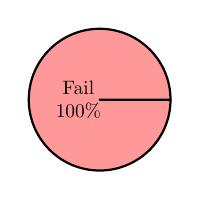
\begin{tikzpicture}[scale=0.3, every node/.style={scale=0.7}]
        \pie [color={green!40, red!40}, text=inside ] {0, 100/Fail}
      \end{tikzpicture}
    \end{minipage}%
     & 
     \begin{minipage}{0.15\textwidth}%
      \centering%
      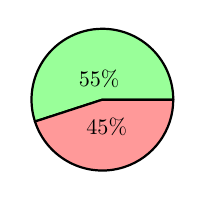
\begin{tikzpicture}[scale=0.3, every node/.style={scale=0.8}]
        \pie [color={green!40, red!40}, text= ] {55/Pass, 45/Fail}
      \end{tikzpicture}
    \end{minipage}%
    & 
    \begin{minipage}{0.15\textwidth}%
     \centering%
     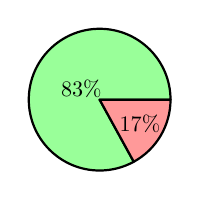
\begin{tikzpicture}[scale=0.3, every node/.style={scale=0.8}]
       \pie [color={green!40, red!40}, text= ] {83/Pass, 17/Fail}
     \end{tikzpicture}
   \end{minipage}%
   & 
   \begin{minipage}{0.15\textwidth}%
    \centering%
    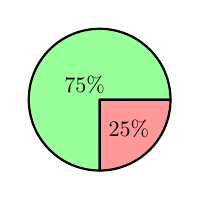
\begin{tikzpicture}[scale=0.3, every node/.style={scale=0.8}]
      \pie [color={green!40, red!40}, text= ] {75/Pass, 25/Fail}
    \end{tikzpicture}
  \end{minipage}%
  \\

     {\huge 4} & 
     \begin{minipage}{0.15\textwidth}%
       \centering%
       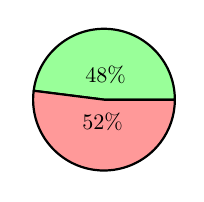
\begin{tikzpicture}[scale=0.3, every node/.style={scale=0.8}]
         \pie [color={green!40, red!40}, text= ] {48/Pass, 52/Fail}
       \end{tikzpicture}
     \end{minipage}%
      & 
      \begin{minipage}{0.15\textwidth}%
       \centering%
       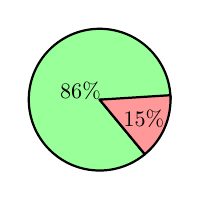
\begin{tikzpicture}[scale=0.3, every node/.style={scale=0.8}]
         \pie [color={green!40, red!40}, text= ] {86/Pass, 15/Fail}
       \end{tikzpicture}
     \end{minipage}%
     & 
     \begin{minipage}{0.15\textwidth}%
      \centering%
      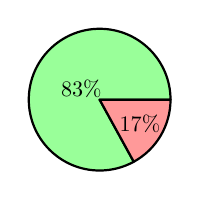
\begin{tikzpicture}[scale=0.3, every node/.style={scale=0.8}]
        \pie [color={green!40, red!40}, text= ] {83/Pass, 17/Fail}
      \end{tikzpicture}
    \end{minipage}%
    & 
    \begin{minipage}{0.15\textwidth}%
     \centering%
     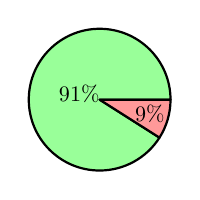
\begin{tikzpicture}[scale=0.3, every node/.style={scale=0.8}]
       \pie [color={green!40, red!40}, text= ] {91/Pass, 9/Fail}
     \end{tikzpicture}
   \end{minipage}%
     \\

      {\huge 5} & 
      \begin{minipage}{0.15\textwidth}%
        \centering%
        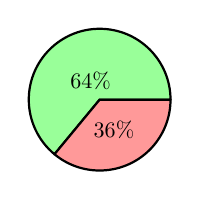
\begin{tikzpicture}[scale=0.3, every node/.style={scale=0.8}]
          \pie [color={green!40, red!40}, text= ] {64/Pass, 36/Fail}
        \end{tikzpicture}
      \end{minipage}%
       & 
       \begin{minipage}{0.15\textwidth}%
        \centering%
        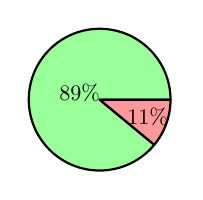
\begin{tikzpicture}[scale=0.3, every node/.style={scale=0.8}]
          \pie [color={green!40, red!40}, text= ] {89/Pass, 11/Fail}
        \end{tikzpicture}
      \end{minipage}%
      & 
      \begin{minipage}{0.15\textwidth}%
       \centering%
       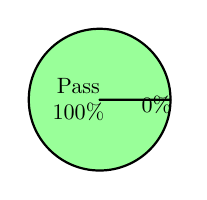
\begin{tikzpicture}[scale=0.3, every node/.style={scale=0.8}]
         \pie [color={green!40, red!40}, text=inside ] {100/Pass, 0/}
       \end{tikzpicture}
     \end{minipage}%
     & 
     \begin{minipage}{0.15\textwidth}%
      \centering%
      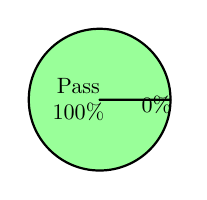
\begin{tikzpicture}[scale=0.3, every node/.style={scale=0.8}]
        \pie [color={green!40, red!40}, text=inside ] {100/Pass, 0/}
      \end{tikzpicture}
    \end{minipage}%
       \\

    \end{tabular}
\end{frame}
}

\begin{frame}[plain]

2016 
\begin{minipage}{0.3\textwidth}%
  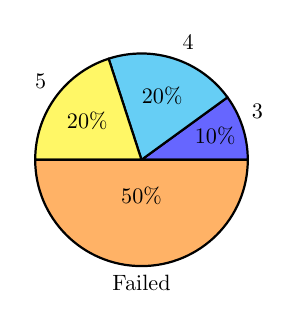
\begin{tikzpicture}[scale=0.45, every node/.style={scale=0.8}]
    \pie{10/3, 20/4, 20/5, 50/Failed}
  \end{tikzpicture}
\end{minipage}%
\begin{minipage}{0.3\textwidth}%
  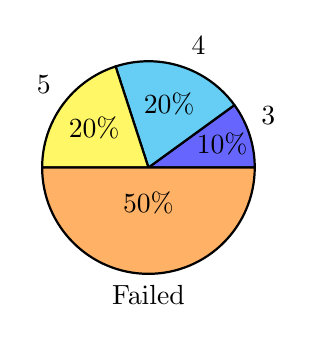
\begin{tikzpicture}[scale=0.45]
    \pie{10/3, 20/4, 20/5, 50/Failed}
  \end{tikzpicture}
\end{minipage}% 
\begin{minipage}{0.3\textwidth}%
  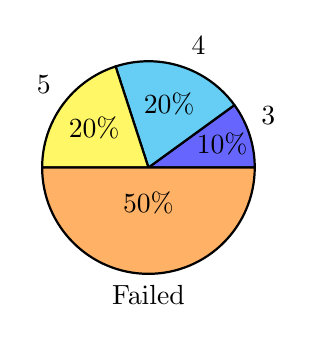
\begin{tikzpicture}[scale=0.45]
    \pie{10/3, 20/4, 20/5, 50/Failed}
  \end{tikzpicture}
\end{minipage}% 

2017
\begin{minipage}{0.3\textwidth}%
  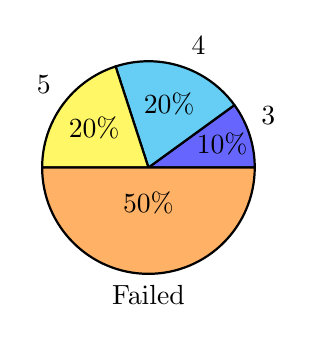
\begin{tikzpicture}[scale=0.45]
    \pie{10/3, 20/4, 20/5, 50/Failed}
  \end{tikzpicture}
\end{minipage}% 

\end{frame}


\begin{frame}[plain]
  \begin{figure}
  \centering
  \begin{tikzpicture}[overlay] 
  \node [] at (0.0mm,-15.0mm) {%
    \includegraphics[height=1.2\paperheight]{Pictures/kids-programming}%
  };
  \end{tikzpicture}%
  \end{figure}%
  \end{frame}%


\begin{frame}[plain]
  \begin{figure}
  \centering
  \begin{tikzpicture}[overlay] 
  \node [] at (0.0mm,-5.0mm) {%
  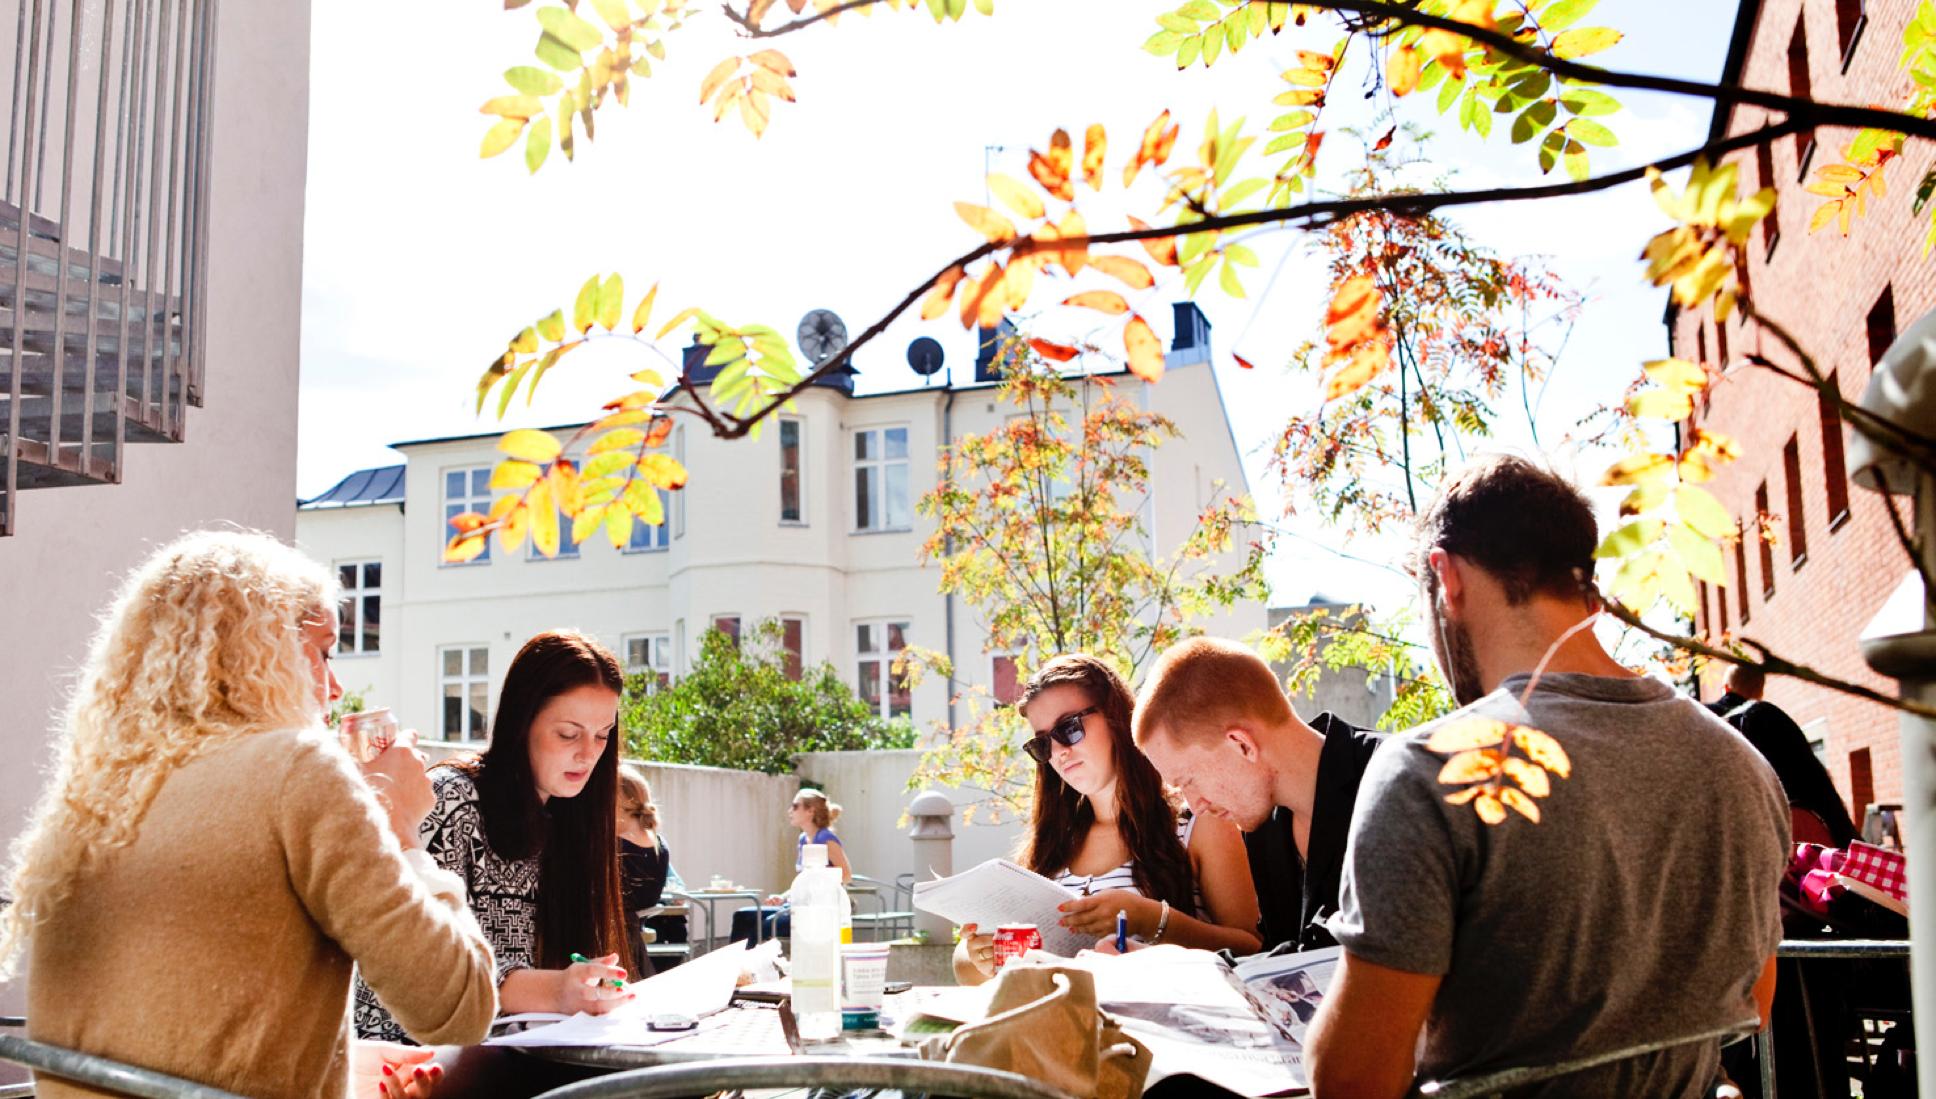
\includegraphics[height=1.2\paperheight]{Pictures/titlepictureGroup}};
  \end{tikzpicture}%
  \end{figure}%
  \end{frame}%

%\begin{frame}[plain]\endpage\end{frame}
 
\End
\end{document}